\documentclass{article}
\usepackage{graphicx}
\usepackage{fullpage}
\title{An overview of the exponential function}
\author{A.T.~Hopkinson}
\date{}
\begin{document}
\maketitle
\section{The exponential function}
The exponential function is a relation in the form $y=a^x$ with the variable x ranging over the entire real numberline. The most important function is $y=e^x$ also written as $y=exp(x)$. In these equations e = 2.7182818... and is the base of the natural logarithm ln.
With the constant e, the constant of proportionality is 1 and the function is its own derivitive.

\section{Expansion and approximation of the exponential function}
The exponential function can also be represented as a Taylor series in an expanded form as can be seen in (\ref{eq:taylor}).

	\begin{equation}\label{eq:taylor}
\exp(x)\equiv\sum_{k=0}^{k=\infty}\frac{x^k}{k!}
	\end{equation}

This representation may be useful due to it allowing for any precision to be used as and when wanted/needed by a system. It would also work better for certain exponentials as the computer can only add, subtract, multiply or divide which makes processing it easier in this format.
The implimentation of this is shown in the code in the next section where I discuss how the code works.

\section{The Code}
double ex(double x)\\
	if(x<0)return 1/ex(-x);\\
	if(x>1./8)return pow(ex(x/2),2);\\
	return 1+x*(1+x/2*(1+x/3*(1+x/4*(1+x/5*(1+x/6*(1+x/7*(1+x/8*(1+x/9*(1+x/10)))))))));\\

This code firstlly checks if the value x is a negative and if it is then it runs the funtion again but does 1/ex(-x). This means it returns the inverse of the function but with a negative value. THis is important because it increases the precision of the value due to making the sums non alternating.

If this is not the case it checks if x is larger than 1/8 and if it is it returns the function of the x value/2 squared. The reason for these size checks is that the precisions of the sum are most accurate the closer to 0 it is. So here for example it will only calculate the taylor series once it has gotten smaller than 1/8. 

After this is done the expanmsion can be calculated. As can be seen it is in a different format to the usual definition but this is due to it removing the indercies and the fractorals which increases the speed of the calculation due to reasons we have previosusly discussed. This results in a approximation of the exponetial function with some advantages to doing it this way.

\section{Comparison}
The bast way to prove that this works in practise and not just theory is to run the code and then plot it. So here is a plot that has both the code given above and the inbuilt exponential function (\ref{fig:plot})
	
\begin{figure}\label{fig:plot}
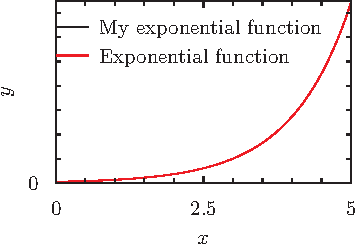
\includegraphics{fig-pyxplot.pdf}
\caption{This plot shows our own exponential function and the computers exponential function.}
\end{figure}



\begin{thebibliography}{9}

\end{thebibliography}

\end{document}
